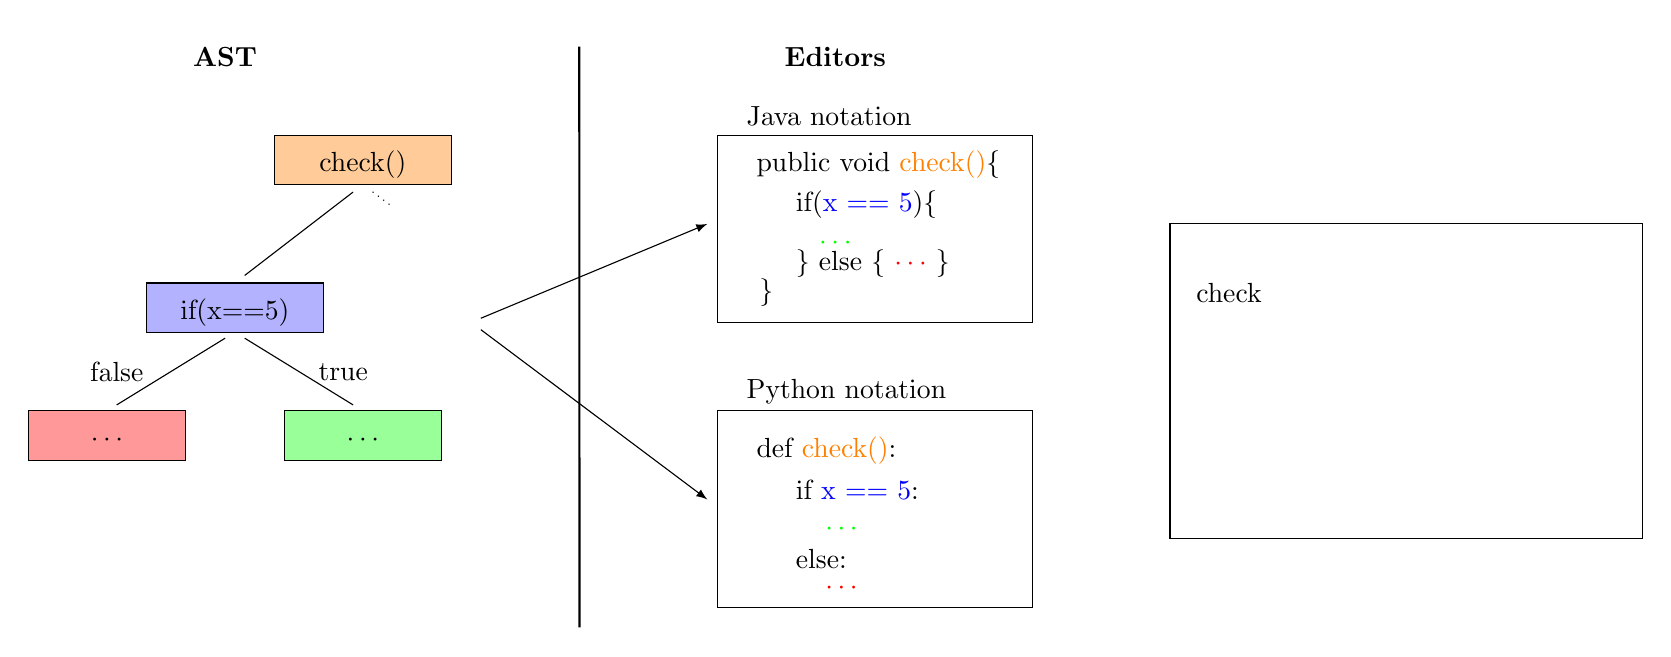
\begin{tikzpicture}


\draw[fill=blue!30]  (-1.125,0.25) rectangle (1.125,-0.375);

\draw[fill=green!40]  (0.625,-1.375) rectangle (2.625,-2);

\draw[fill=red!40]  (-2.625,-1.375) rectangle (-0.625,-2);
\node (v2) at (-1.625,-1.375) {};
\node (v3) at (1.625,-1.375) {};
\node (v1) at (0,-0.375) {};
\draw  (v1) edge (v2);
\draw  (v1) edge (v3);
\node at (1.375,-0.875) {true};
\node at (-1.5,-0.875) {false};

\draw[fill=orange!40]  (0.5,2.125) rectangle (2.75,1.5);
\node (v4) at (1.625,1.5) {};
\node (v5) at (0,0.25) {};
\draw  (v4) edge (v5);

\node (v6) at (2.125,1.125) {};
\draw  (v4) edge[dotted] (v6);



\node at (1.625,1.75) {check()};
\node at (0,-0.125) {if(x==5)};
\node at (-1.625,-1.75) {$\cdots$};
\node at (1.625,-1.75) {$\cdots$};



\node at (-0.125,3.125) {\textbf{AST}};


\node[right] at (6.5,1.75) {public void \textcolor{orange}{check()}\{};
\node[right] at (7,1.25) {if(\textcolor{blue}{x == 5})\{};
\node at (7.625,0.75) {\textcolor{green}{$\cdots$}};
\node[right] at (7,0.5) {\} else  \{ \textcolor{red}{$\cdots$} \}};
\node at (6.75,0.125) {\}};
\draw  (6.125,2.125) rectangle (10.125,-0.25);
\node[right] at (6.375,2.375) {Java notation};


\node [right] at (6.5,-1.875) {def \textcolor{orange}{check()}:};
\node [right] at (7,-2.375) {if \textcolor{blue}{x == 5}:};
\node [right] at (7.375,-2.875) {\textcolor{green}{$\cdots$}};
\node [right] at (7,-3.25) {else:};
\node [right] at (7.375,-3.625) {\textcolor{red}{$\cdots$}};
\draw  (6.125,-1.375) rectangle (10.125,-3.875);
\node [right] at (6.375,-1.125) {Python notation};

\node at (7.625,3.125) {\textbf{Editors}};
\draw (4.25,3.375) node [right] {} edge[thick] (4.375,-4.125) node [right] {};
\draw (2.875,-0.25) node [right] (v7) {} edge[-latex] (6,1) node [right] {};

\draw (v7) edge[-latex] (6,-2.5) node [right] {};


\draw  (11.875,1) rectangle (17.875,-3);
\node at (12.625,0.125) {check};

\end{tikzpicture}